
To enable future scientific breakthroughs and discoveries, the
next-generation of scientific applications will require exascale
computing performance to support the execution of predictive models
and the analysis of massive quantities of data, with orders of
magnitude higher resolution and fidelity than what is possible in
existing computing infrastructure \cite{sachs_ascr_2011,doe_exascale_2010}. In order to deliver exascale computing and
effectively harness its capabilities, several daunting scalability
challenges must be addressed. In the late 90's, terascale performance
was achieved with fewer than 10,000 single-core processors. A decade
later, petascale performance required about 10 times as many
processors as terascale performance. If such trends continue,
delivering exascale computing will require a million processors, each
supporting 1000 cores, resulting in a billion-core computing
infrastructure with a massive increase in the number of memory
modules, communications devices and storage components. Beyond raw
computing, communications and storage requirements, future exascale
computing systems are faced with unprecedented energy and resiliency
challenges.

Power consumption is widely recognized as one of the most significant
challenges facing exascale computing
\cite{doe_exascale_2010,sachs_ascr_2011}. The expected energy
consumption increase in exascale computing is staggering. If current
trends hold true, an exascale computing system is expected to consume
over a gigawatt of power. This represents a 10 fold increase in the
energy consumption of today's largest data centers, which typically
ranges between 100 and 200 Megawatts. Reducing the power consumption
of an exascale computing system to the DoE's target of 20 Megawatts is
undoubtedly a formidable challenge, with a pervasive effect on next
generation scientific applications. Addressing such a challenge
requires building power and energy awareness into the foundations of
future exascale computing infrastructure, with "performance per watt"
as the metric of merit to measure efficiency. Radical approaches must
be developed to achieve efficient energy management across all
hardware and software components of the system.

In addition to its impact on energy consumption, the upward trend in
the number of computing nodes also has a direct negative effect on the
overall system reliability. Even if the individual node failure rate
is low, the overall system failure rate quickly becomes unacceptable
as the number of components increases. For example, a computing system
with 200,000 nodes will experience a mean time between failure(MTBF)
of less than one hour, even when the MTBF of an individual node is as
large as 5 years \cite{riesen_sandia_2010}. The dramatic decrease in
system reliability as the number of computing nodes increases is
depicted in Figure \ref{sandia_system_mtbf}
\cite{riesen_sandia_2010}. Other factors are also expected to increase
failure rates in exascale computing, including the expected high fault rates of
advanced-technology computing components operating at lower voltage
levels and the impact of undesirable aging effects as they become
significant\cite{srinivasan_dsn_2004}. Addressing these concerns
brings about unprecedented resiliency challenges, which puts in
question the ability of next generation high performance computing to
continue operation in the presence of faults without compromising the
requirements of the supported applications.

\begin{figure}[!t]
\centering
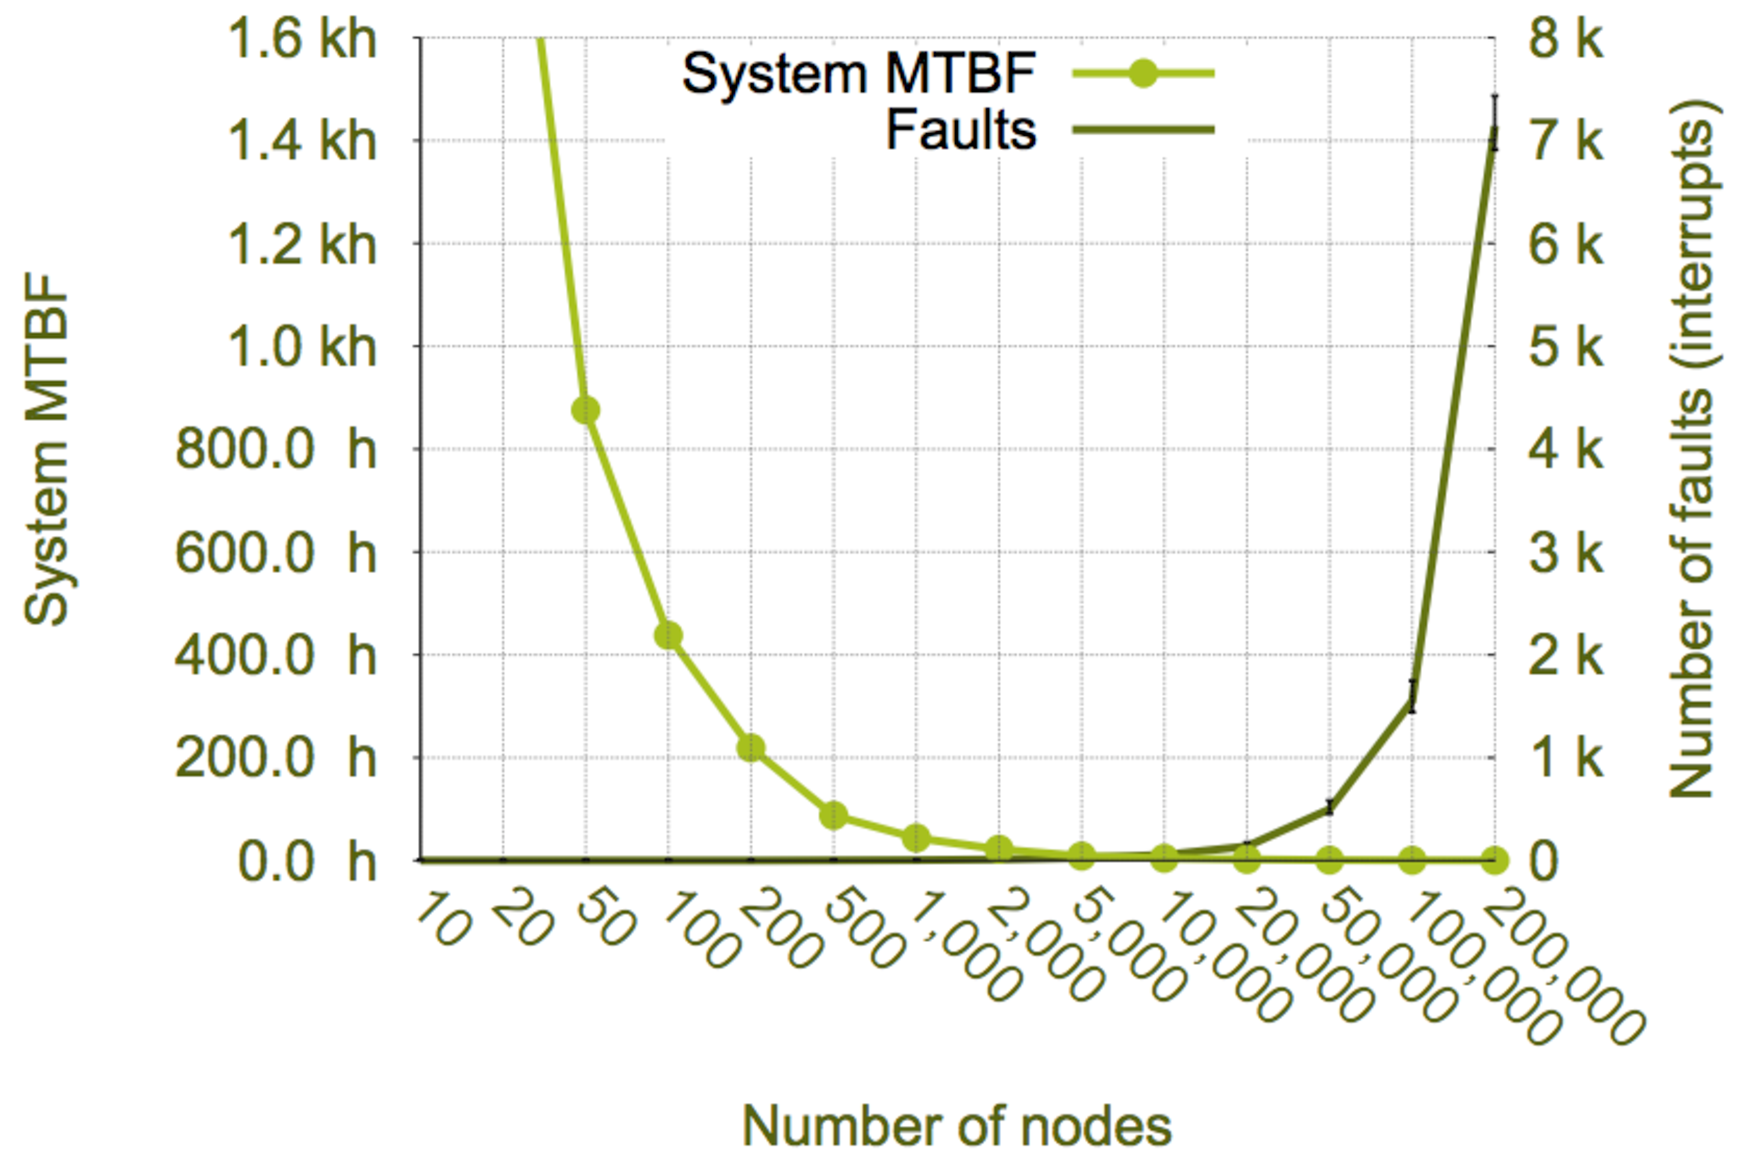
\includegraphics[width=\columnwidth]{figures/sandia_system_failure_rate_increase_nodes.pdf}
%\psfig{figure=diagrams/sandia_system_failure_rate_increase_nodes.eps,width=3.0in}
\caption { Effect on system MTBF as number of nodes increase. }
\label{sandia_system_mtbf}
\end{figure}

The current response to faults consists of restarting the execution of
the application, including those components of its software
environment that have been affected by the occurring fault. To avoid
the full re-execution of the failing application, fault-tolerant
techniques typically checkpoint the execution periodically; upon the
occurrence of a hardware or software failure, recovery is achieved by
restarting the computation from a safe checkpoint. In some situations,
however, several components of the software environment associated
with the failed application may have to be restarted.

Given the anticipated increase in failure rate and the time required
to checkpoint large-scale compute- and data-intensive applications, it
is very likely that the time required to periodically checkpoint an
application and restart it upon failure may exceed the mean time
between failures.  Consequently, applications may achieve very little
computing progress, thereby reducing considerably the overall
performance of the system.  For example, a study carried out at Sandia
National Laboratories focused on evaluating the overhead incurred by
checkpointing in exascale computing environments. The results of the
study, depicted in Figure \ref{sandia_checkpoint_time}, clearly show
that beyond 50,000 nodes the application spends only a fraction of the
elapsed time performing useful computation.

\begin{figure}[!t]
\centering
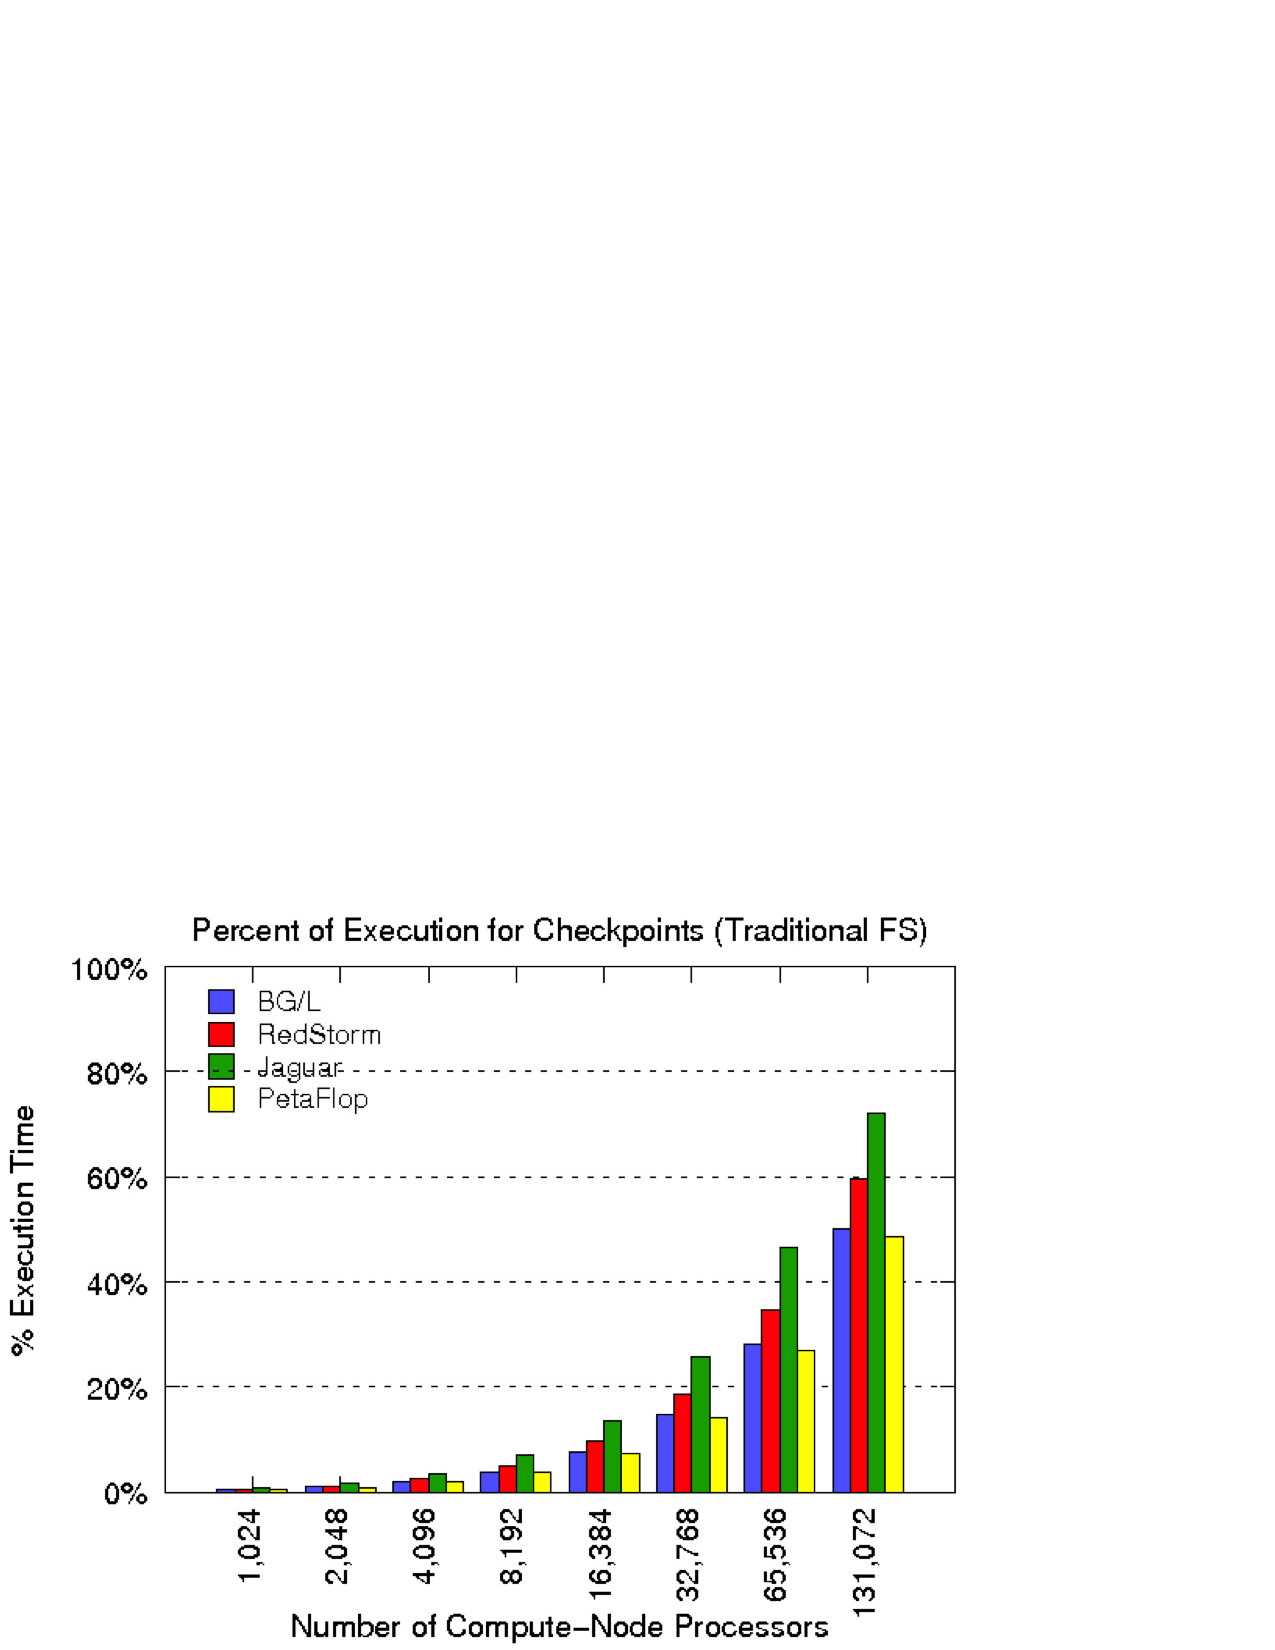
\includegraphics[width=\columnwidth]{figures/sandia_percent_of_time_for_checkpoints.pdf}
%\psfig{figure=diagrams/sandia_percent_of_time_for_checkpoints.eps,width=3.0in}
\caption { Percent of time to perform checkpoints. }
\label{sandia_checkpoint_time}
\end{figure}


The main objective of this paper is to explore radically different
paradigms to enable scalable resiliency with minimum energy
consumption in the future exascale computing infrastructure. To this
end, we propose a new energy-aware ``shadow computing'' model, as the
basis for an efficient and scalable computational framework to achieve
desired levels of fault tolerance, while minimizing energy
consumption. The proposed model goes beyond traditional check-pointing
and roll-back recovery techniques, and uses a multi-level,
energy-aware replication approach to achieve scalable fault tolerance
in exascale computing.

The basic idea of the shadow computing model is to associate with each
process a suite of ``shadow processes'', whose size depends on the
``criticality'' and performance requirements of the underlying
application. A shadow is an exact replica of the main process. In
order to overcome failure, the shadow is scheduled to execute
concurrently with the main process, but at a different computing
node. Furthermore, in order to minimize energy, shadow processes
initially execute at decreasingly lower processor speeds. The
successful completion of the main process results in the immediate
termination of all shadow processes. If the main process fails, however,
the primary shadow process immediately takes over the role of the main
process and resumes computation, possibly at an increased speed, in
order to complete the task. Moreover, one among the remaining shadow processes
becomes the primary shadow process.

It is worth noting that, since the failure of an individual component
is much lower than the aggregate system failure, it is very likely
that most of the time the main processes complete their execution
successfully. Successful completion of a main process automatically
results in the immediate halting of its associated shadow processes,
with a significant saving in energy consumption. Furthermore, the number
of shadow processes to be instantiated in order to achieve the desired level
of fault-tolerance must be determined based on the likelihood that
more one process failure within the execution time interval of the main
task.

The main challenge in realizing the
potential of the shadow computing model stems from the need to compute
the speed of execution of the main process and the speed of execution
of its associated shadows, both before and after a failure occurs, so
that the target response time is met, while minimizing energy
consumption. Given the nature of failure in exascale
computing, it is unlikely that both the main and its primary shadow
fail simultaneously. Therefore, only a dual level of redundancy,
whereby only one shadow process is executed concurrently with the main
process, is needed in most cases to achieve the desired level of
fault-tolerance. The completion of a main or its shadow results in the
successful execution of the underlying task.

The main contributions of this paper are threefold. First, we present
an optimization framework to explore the applicability of the shadow
computing model to support fault-tolerance in a high-performance
computing environment, where the main computation is expected to
execute at maximum speed in order to harness the full potential of the
computing infrastructure. The model assumes that the desired level of
fault tolerance can be achieved with the instantiation of a single
shadow process, although the model can be extended to support multiple
shadow processes.  

Second, using the optimization framework, we propose and study three
implementation methods of the shadow computing model. The first
method, referred to as ``stretched'' replication, takes a
straight-forward approach to minimizing energy by computing a uniform
speed of execution across the execution interval.  Although simple to
implement, stretched replication is oblivious to the dynamics of the
failure, resulting in sub-optimal energy performance.  The second
method, referred to as minimum-work replication, takes into
consideration the minimum time between failures for a single node is
likely to exceed the execution time of the task. Based on this
observation, the method computes a near-optimal execution speed of the
shadow. The third method, referred to as optimal energy replication,
addresses shortcomings in these two models and uses an optimal
energy-consumption approach to derive the shadow's minimum-energy
speed, both before and after failure, in order to meet the expected
response time of the underlying application regardless of failure
rates. It is worth noting that the implementation complexity of the
optimal approach does not increase significantly in comparison with
the stretched and minimum-work replication schemes.

Third, we propose a performance evaluation framework to assess the
performance of the proposed methods for different workload
characteristics and performance requirements of the main
task. Throughout the study, the performance of the proposed shadow
computing implementation methods are compared to that of the ``pure''
replication scheme described in
\cite{ferreira_hpc_2011}. The major difference between the methods
proposed in this paper and current replication schemes is that shadow
computing does not force the process replica to execute at the same
speed as the main process. As the results of the performance study
show, relaxing this restriction allows shadow computing to save up to
50\% of the expected energy consumed by pure replication.

The remainder of the paper is organized as follows: Section
\ref{related_work} reviews work related to fault-tolerance in
large-scale high-performance computing systems. Section
\ref{shadow_model} presents the shadow computing model and discusses
the building components of its execution model. Section \ref{model}
the shadow computing model is cast as an energy optimization problem
to achieve fault-tolerance, while minimizing energy consumption
without violating the expected performance requirements of the
supported application. In Is Section 5 three different approaches to
solving the energy optimization problem and their potential
implementation are explored. The methods differ in their approach to
energy minimization and their reaction to failures. In Section
\ref{analysis}, we develop a performance evaluation framework to
analyze and assess the performance of the three shadow computing
methods, including their sensitivity to critical workload and
performance parameters.  Throughout the study, the performance of the
three methods is compared to pure replication, a recently proposed
alternative to check-pointing in exascale computing.  Section
\ref{conclusion} presents the conclusion of this work and discusses
future work.
